\chapter{Contesto e motivazioni}
\section{Scenario}
Nell'ambiente in cui viviamo siamo circondati da sempre più entità
computazionali eterogenee tra loro. Device come smartphone, smartwatch, fitness
tracker, display pubblici, droni, insegne digitali, sensori di ogni tipo stanno
sempre più pervadendo il nostro ambiente quotidiano. L'interazione tra questi
dispositivi gioca un ruolo fondamentale in settori emergenti come
Internet-of-Things (IoT), Smart City, reti di sensori o più in generale in
sistemi collettivi adattivi. Quando si parla di sistemi collettivi si deve
tenere in considerazione l'elevato numero di dispositivi diversi di cui essi
sono composti e l'eterogeneità che ne deriva in termini di piattaforme,
tecnologie, paradigmi di programmazione, protocolli di comunicazione,
eccetera. Specifiche come efficienza, organizzazione e la necessità di
coordinare i dispositivi, influenzano pesantemente le scelte di design del
sistema, che può risultare rigido, costoso da manutenere, estendere, ed
eventualmente scalare in dimensione.

Sorge quindi la necessità di un modello di programmazione più ad alto livello,
che consenta di astrarre i dettagli di un sistema e possa occuparsi di tutti i
requisiti non funzionali come le proprietà di auto-organizzazione e
auto-adattività, delegando allo strato sottostante tutte le questioni di più basso livello. Possono essere elencate tre caratteristiche
chiave che questo strato dovrebbe presentare\cite{DBLP:journals/computer/BealPV15
}:
\begin{itemize}
\item i meccanismi di comunicazione dovrebbero essere nascosti e i gli
  sviluppatori non dovrebbero essere tenuti a interagire con essi;
\item la composizione di moduli o sottosistemi dovrebbe essere semplice e
  trasparente;
\item sottosistemi distinti necessitano di meccanismi di coordinazione per
  distinte regioni dello spazio-tempo.
\end{itemize}

\begin{figure}
  \centering
  \includegraphics[width=\linewidth]{images/streetscene}
  \caption{Lo spazio che ci circonda è denso di oggetti in grado di effettuare
    calcoli e capaci di comunicare. Alcuni di questi sono oggetti
    infrastrutturali, ma la maggior parte sono oggetti personali, in continuo
    movimento. Immagine tratta da \cite{Protelis}.}
  \label{fig:streetscene}
\end{figure}

\section{Aggregate computing}
\label{sec:aggregate-computing}
\begin{figure}
  \subfloat[Programmazione device-centric]{
    \includegraphics[width=\linewidth]{images/distributed-composition}
    \label{fig:device-centric}
  }\hfill
  \subfloat[Programmazione aggregata]{
    \includegraphics[width=\linewidth]{images/aggregate-composition}
    \label{fig:aggregate-computing}
  }
  \caption{Differenze tra programmazione orientata al singolo dispositivo e
    programmazione aggregata. Immagini tratte da \cite{Protelis}.}
\end{figure}
Spesso la modellazione del comportamento collettivo di un sistema interessa più
del singolo dispositivo di cui è composto, ma i linguaggi di programmazione
classici, orientati al singolo dispositivo, forzano lo sviluppatore a porre
l'attenzione sui singoli device e all'interazione tra di
essi. L'\textit{aggregate computing} è un paradigma che si propone di risolvere
le precedenti questioni tramite i seguenti
principi\cite{DBLP:journals/computer/BealPV15}:
\begin{enumerate}
\item il dispositivo programmato è una regione dell'ambiente computazionale e
  prescinde dagli specifici dettagli;
\item il programma è specificato come manipolazione funzionale di strutture dati
  distribuite nello spazio-tempo di interesse;
\item queste manipolazioni sono effettivamente eseguite dai singoli dispositivi
  nella regione, usando meccanismi di coordinazione resilienti e interazioni
  basate sulla prossimità.
\end{enumerate}

Un esempio di utilizzo nel mondo reale potrebbe essere un servizio che,
utilizzando interazioni tra gli smartphone per stimare la densità di popolazione
presente in un area o ad un certo evento, possa fornire indicazioni relative a
zone che possono essere considerate pericolose perché troppo dense e che percorso
seguire eventualmente per disperderle; più in generale, possono essere erogate
indicazioni per raggiungere un punto scelto evitando le zone più pericolose.

La Figura \ref{fig:device-centric} mostra come con un linguaggio di
programmazione orientato al singolo device il programmatore sia costretto a
porre la propria attenzione sull'interazione tra i dispositivi, mentre si occupa
di modellare localmente un comportamento che dovrà produrre un certo effetto
globale.  Invece, con l'utilizzo della programmazione aggregata (Figura
\ref{fig:aggregate-computing}), si è liberi di pensare in maniera più naturale
tramite strutture dati \textit{continuum-like} e servizi che possono essere
composti in maniera modulare.  Nello specifico il servizio di \textit{crowd
  estimation} produce in output una struttura dati distribuita --- un campo
computazionale --- che associa ad ogni posizione una densità di
popolazione. Questo è l'input dei servizi che poi si vogliono costruire:
navigazione, segnalazione delle zone di pericolo ed istruzioni per un'eventuale
evacuazione.

La capacità di separare la logica dei servizi dall'implementazione della
comunicazione e dai protocolli utilizzati per questa, orientano verso lo
sviluppo di applicazioni distribuite più complesse, ma allo stesso tempo
modulari, riusabili e facilmente estendibili.

L'obiettivo della programmazione aggregata è nascondere la complessità di
coordinare un sistema distribuito utilizzando diversi livelli di astrazione.
Nel tempo sono stati sviluppati diversi modelli di programmazione aggregata, ma
la maggior parte di questi si sono rivelati troppo specializzati per singole
istanze di problemi e non sufficientemente generici da risolvere intere classi
di questi\cite{beal2012}. Un'eccezione è il \textit{field calculus}: un insieme
di costrutti fondamentali, derivati dagli elementi comuni degli altri metodi,
che modellano la computazione e l'interazione tra un largo numero di dispositivi
sparsi nello spazio.

% TODO figura 1
% https://ieeexplore.ieee.org/stamp/stamp.jsp?tp=&arnumber=8064162
\subsection{Field calculus}
Utilizzando diversi approcci di programmazione aggregata emergono pattern
ripetitivi. Il \textit{field calculus} \cite{Viroli2013} ne riassume le
caratteristiche dei suddetti pattern in una semantica operazionale minimale che
da origine ad un linguaggio universale\cite{spacetime}.

L'elemento fondamentale del \textit{field calculus} è il campo computazionale,
ispirato a concetti fisici come i campi magnetici, che associa ad ogni
dispositivo in rete un valore locale. Ogni valore, funzione o variabile è un
campo: per esempio una collezione di sensori di temperatura produce un campo di
temperature dell'ambiente, una collezione di accelerometri di smartphone produce
un campo di direzioni, una notifica di un'applicazione produce un campo di
messaggi.

I campi sono generati e manipolati utilizzando quattro costrutti fondamentali:
\begin{itemize}
\item \textbf{Funzione}: \texttt{b($e_1,\ldots, e_n$)} applica la funzione \texttt{b}
  agli argomenti \texttt{$e_1,\ldots, e_n$}. Queste sono funzioni matematiche,
  logiche o algoritmiche stateless, oppure sensori, attuatori, funzioni definite
  dall'utente o importate da librerie.

\item \textbf{Dinamica e stato}: \texttt{rep(x<-v) \{$s_1;\ldots;s_n$\}} definisce una variabile
  locale di stato \texttt{x} inizializzata con il valore \textit{v} e aggiornata
  periodicamente con il risultato dell'esecuzione gli statement
  \texttt{{$s_1;\ldots;s_n$}} che compongono il suo corpo. In questo modo viene
  definito un campo che cambia nel tempo.

\item \textbf{Interazione}: \texttt{nbr($s$)} acquisisce un campo che associa ad ogni
  device tra tutti i dispositivi vicini (incluso se stesso), il loro ultimo
  valore di \texttt{$s$}. Questo campo può essere poi processato da funzioni
  built-in chiamate \textit{hood}, che permettono di ridurre il campo ad un
  valore, per esempio il minimo.

\item \textbf{Restrizione del dominio}: \texttt{if($e$) \{$s_1;\ldots;s_n$\} else
    \{$s'_1;\ldots;s'_m$\}} partiziona la rete in due regioni disgiunte: dove la
  \texttt{$e$} è vero viene eseguito \texttt{$s_1;\ldots;s_n$}, nell'altra parte,
  invece, è eseguito \texttt{$s'_1;\ldots;s'_n$}. È importante menzionare il
  fatto che le due diramazioni sono incapsulate e non possono avere effetti al
  di fuori del loro sottospazio.
\end{itemize}

Questi costrutti permettono portabilità, indipendenza dall'infrastruttura e
modularità.

\subsection{Building blocks}
\begin{figure}
  \centering
  \includegraphics[width=\linewidth]{images/layers-cropped}
  \caption{Livelli di astrazione dell'aggregate computing. A basso livello le
    capacità software e hardware vengono astratte e composte per creare un
    livello comune: il \textit{field calculus}, che è la base di
    partenza dell'architettura delle API. Immagine tratta da \cite{Protelis}.}
  \label{fig:abstraction-layers}
\end{figure}

Il successivo livello di astrazione serve ad aggiungere resilienza. È
identificata una collezione di operatori ``building block'' generici finalizzata
a una coordinazione robusta delle applicazioni. I meccanismi di questo livello
(quello in mezzo nella Figura \ref{fig:abstraction-layers}), sono
\textit{auto-stabilizzanti}, cioé raggiungono lo stato corretto
indipendentemente dallo stato di partenza in un numero finito di passi,
caratteristica che preservano quando sono composti tra loro\cite{7056345}.

La collezione è composta da tre operatori di coordinazione generali, che
mascherano gli elementi di basso livello del linguaggio, e dal costrutto
\texttt{if}. I tre operatori sono:
\begin{itemize}
\item \texttt{G(source, init, metric, accumulate)}: distribuisce un
  informazione nello spazio. Questo operatore generalizza operazioni molto
  comuni come la stima della distanza e messaggi broadcast. Per farlo esegue due
  azioni: computa un campo di distanze minime da una regione \texttt{source}
  utilizzando la \texttt{metric} scelta; in seguito propaga i valori attraverso
  i nodi iniziando da \texttt{init} e modificandolo con la funzione
  \texttt{accumulate}.
\item \texttt{C(potential, accumulate, local, null)}: aggrega un'informazione
  alla \texttt{source} attraversando il gradiente di un campo
  \texttt{potential}. Viene effettuata una riduzione che, iniziando con il
  valore \texttt{null} e sfruttando una funzione associativa
  \texttt{accumulate}, risale il gradiente verso la \texttt{sorgente} e combina
  i valori in \texttt{local}.
\item \texttt{T(init, floor, decay)}: generalizza un timer il cui rateo di
  aggiornamento può variare nel tempo. La funzione \texttt{decay} diminuisce il
  valore del proprio input successivo, che parte da \texttt{initial} e si ferma
  a \texttt{floor}.
\end{itemize}
\begin{figure}
  \centering
  \subfloat[Operatore G]{
    \includegraphics[]{images/op-G}
    \label{fig:op-g}
  }
  \subfloat[Operatore C]{
    \includegraphics[]{images/op-C}
    \label{fig:op-g}
  }\hfill
  \subfloat[Operatore T]{
    \includegraphics[]{images/op-T}
    \label{fig:op-g}
  }
  \subfloat[Operatore if]{
    \includegraphics[]{images/if}
    \label{fig:op-g}
  }\hfill
  \caption{``Building block'' per computazioni aggregate: questi quattro
    operatori sono la base fondante di tutte le API auto-stabilizzanti fornite
    al livello superiore. Immagini tratte da \cite{Protelis}.}
\end{figure}


\subsection{General-purpose API}
È un ulteriore livello di astrazione (il secondo dall'alto nella Figura
\ref{fig:abstraction-layers}) che mira a semplificare la composizione dei
building-blocks, fornendo delle API di alto livello\cite{amslaurea13090}: funzioni come
\texttt{distanceTo}, che permette di ottenere la distanza tra nodi utilizzando
una data metrica, o \texttt{broadcast}, che consente di diffondere un messaggio
nella rete.

Queste API possono essere usate e composte tra loro per scrivere applicazioni
distribuite senza proccuparsi di meccanismi di coordinazione. Infatti costruire
delle API utilizzando degli operatori \textit{resilient} assicura che i servizi
lo siano a loro volta.

Inoltre sono esposti da questo livello dei meccanismi di coordinazione non
auto-stabilizzanti, utili in determinati ambiti applicativi.

\section{Protelis}
Il \textit{field calculus} è un fondamento teoretico importante, ma manca di uno
strumento pratico che fornisca tool, librerie e possibilità di integrazione con
piattaforme esistenti. Protelis\cite{Protelis} è un linguaggio di programmazione
che si pone come obiettivo quello di fornire un'implementazione pratica
dell'\textit{higher-order field calculus}\cite{Audrito:2019:HCC:3301291.3285956}
con la capacità di interfacciarsi con hardware, sistemi operativi e piattaforme
esistenti. Poiché la maggior parte dei sistemi che saranno implementati tramite
questo linguaggio saranno distribuiti, è di fondamentale importanza che
l'implementazione sia facilmente portabile tra un ambiente simulato, nel quale
un'applicazione può essere testata, e un ambiente reale, dove questa potrà
essere eseguita in produzione.

La sintassi del linguaggio è di facile apprendimento in quanto si ispira a
quella dei linguaggi C-like come Java.

\subsection{Protelis nel mondo scientifico}
Protelis è in grado di esprimere algoritmi distribuiti complessi in poche righe
di codice. È infatti stato sfruttato per implementare diversi algoritmi
distribuiti. Tra questi i più rilevanti sono: \textit{rendezvous} ad una
riunione di massa\cite{Protelis}, algoritmo che consente a due persone che
partecipano ad un evento di massa di incontrarsi in un punto intermedio,
evitando zone di alta densità; stima di pericolosità di una zona per
sovrappopolazione e notifica di pericolo\cite{7056345}, che consente di stimare
la pericolosità di una zona, basandosi sulla densità di dispositivi presenti in
essa, e come disperdere l'eventuale massa di persone in maniera efficiente.

Un altro ambito di utilzzo è la gestione dei servizi in una rete:
alcuni servizi di rete sono spesso \textit{legacy} e possono non essere in
grado di gestire un errore degli altri servizi da cui dipendono. Quindi
potrebbero continuare a comportarsi in maniera non definita, modificando in
maniera inconsistente il proprio stato. Reagire in maniera coerente ad un errore
del genere richiede un sistema di coordinazione tra i servizi coinvolti per
riavviare l'intero stack. La programmazione aggregata è stata usata per
risolvere il problema in \cite{7306601}.

La realtà aumentata, AR, è un ambito nel quale sono stati fatti tentativi di
integrazione con la programmazione aggregata, poiché sono settori di ricerca che
hanno in comune l'interazione con l'ambiente reale. In \cite{7306561} viene
introdotto il concetto di campi aumentati, una combinazione di campi
computazionali e realtà aumentata. Le possibili applicazioni dei campi aumentati
sono la visualizzazione dei campi computazionali tramite visori, o l'interazione
dei campi con dati prodotti AR.

Altri contesti in cui Protelis è stato utilizzato sono coordinazione di
droni\cite{7789463}, sensor sharing\cite{Beal:2018:AOA:3208359.3179994} e task
allocation\cite{8791999}.

\subsection{Architettura di Protelis}\label{subsec:Architettura di Protelis}
\begin{figure}
  \subfloat[Funzionamento di Protelis]{
    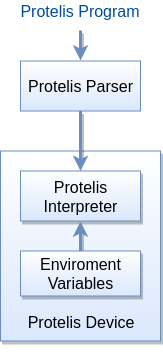
\includegraphics[height=6.8cm]{images/protelis-architecture.png}
    \label{fig:architettura-protelis}
  }\hfill
  \subfloat[Estendibilità di Protelis]{
    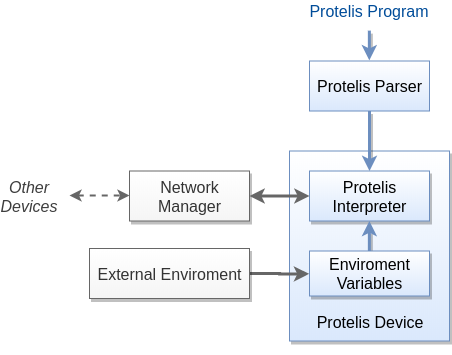
\includegraphics[height=6.8cm]{images/extend-protelis.png}
    \label{fig:estensione-protelis}
  }
  \caption{Architettura astratta di Protelis (a) e meccanismo di estendibilità
    previsto dal linguaggio (b). Immagini tratte da \cite{Protelis}.}
\end{figure}

Protelis è un linguaggio di programmazione aggregato, fortemente influenzato da
Proto\cite{Proto}, la cui esecuzione avviene all'interno di una macchina
virtuale\cite{Protelis}.  Inizialmente un parser traduce un programma Protelis
in una rappresentazione comprensibile all'interprete, che può eseguirlo, in
seguito, a intervalli regolari. L'interprete può interagire con l'ambiente
circostante, implementato tramite coppie \textit{(chiave, valore)} (Figura
\ref{fig:architettura-protelis}).

La duplice possibilità di poter eseguire un interprete Protelis in due contesti
diversi, quali sono un ambiente simulato e quello reale, evidenziano la
necessità dell'introduzione di un componente middleware, che gestisca la
comunicazione tra le macchine virtuali in maniera completamente trasparente a
queste ultime (Figura \ref{fig:estensione-protelis}). Sfruttando la
caratteristica del polimorfismo dei linguaggi ad oggetti, questo modello può
essere facilmente specializzato in entrambi i contesti precedentemente citati.

La piattaforma di supporto scelta per l'implementazione è Java, scelta per la
sua portabilità, il meccanismo interno della reflection, e il sempre crescente
numero di dispositivi embedded a basso costo che supportano Java. Un altro
fattore determinante è l'efficienza in termini di costo di risorse che le
implementazioni Java hanno raggiunto, rendendolo competitivo con linguaggi di
basso livello come C o C++.

Protelis è interoperabile con Java, e indirettamente con Kotlin, di conseguenza
può essere integrato con un vastissimo ecosistema di librerie.
